\chapter{Introduction}

\iffalse
	\begin{wrapfigure}[12]{l}{5cm}
	\vspace{-5mm}
	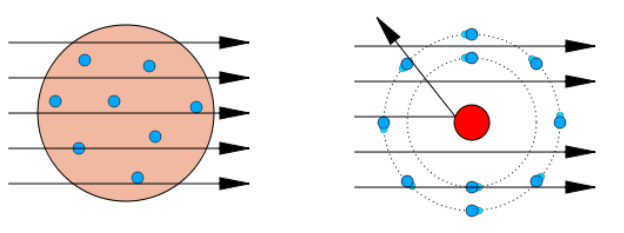
\includegraphics[scale=0.1]{ch1/image1.png}
	\captionof{figure}{ }
	\end{wrapfigure}
\fi	

\section{Historique}
	\begin{wrapfigure}[10]{r}{7.5cm}
	\vspace{-5mm}
	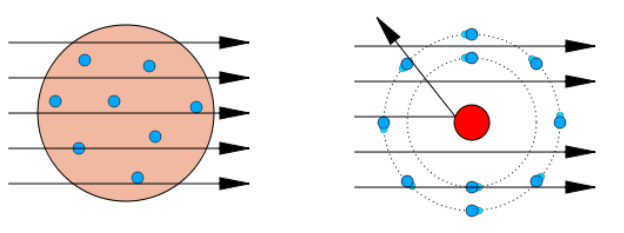
\includegraphics[scale=0.35]{ch1/image1.png}
	\captionof{figure}{A gauche le modèle de \textsc{Thompson} et à droite celui de \textsc{Rutherford}.}
	\end{wrapfigure}
Le premier modèle nucléaire a été proposé par \textsc{Thompson} en \textit{1904} : le modèle du 
\textit{plumb-pudding} qui voit l'atome comme formé d'une charge positive et des électrons\footnote{Découvert 
eux en \textit{1897}.}. C'est en \textit{1911} que \textsc{Rutherford} établit l'existence du noyau. En 
bombardant une feuille d'or de particules $\alpha$ il a remarqué que peu d'entre elles sont déviées, 
confirmant la présence d'une charge positive dans un faible volume.\\

En \textit{1913}, \textsc{Bohr} annonça que les électrons gravitent autour du noyau et c'est de nouveau
\textsc{Rutherford} qui en \textit{1919} établit la \textit{réaction de transfert} 
\begin{equation}
\ ^{13}N+\alpha\to\ ^{17}O+p
\end{equation}
Un an plus tard, en \textit{1920}, \textsc{Eddington} suggère que cette relation prend place dans les 
étoiles. La découverte du neutron vient en \textit{1932} par \textsc{Chadwick}
\begin{equation}
\ ^9\text{Be} + \alpha\to\ ^{12}\text{C}+n
\end{equation}
Celle-ci résulte d'un rayonnement très pénétrant et met en évidence la structure du noyau en protons et 
neutrons.

Peu d'entre-elles étaient déviée, et pourtant la densité nucléaire est très importante.


\newpage
\section{Unité, ordre de grandeur}
La taille typique d'un noyau est de $10^{-15}$ m, beaucoup plus petit que l'atome qui a une taille 
de l'ordre de l'angström ($1 \mathring{A}=10^{-10}$ m), ce qui leur donne des densités bien différentes

\notes{Calculons la densité nucléaire. La masse d'un atome s'exprime
\begin{equation}
m_{at} = m_N + m_E \approx m_N
\end{equation}
Connaissant les tailles respectives, on sait que $\rho_N/\rho_A \approx 10^{15}$ et donc
\begin{equation}
\rho_N\approx 10^{15}\text{ g.cm$^{-3}$},\qquad\qquad\qquad\rho_A\approx 1\text{ g.cm$^{-3}$}
\end{equation}
Notons que la densité nucléaire $\rho_N$ est propre aux étoiles à neutrons. 
}\ \\

L'énergie typiquement utilisée est celle d'1 MeV, soit $10^6$ eV ou encore 1.602*$10^{-13}$ J. Les 
trois relations suivantes permettent de retrouver ces deux unités par simple multiplication
\begin{enumerate}
\item Masse : $m\to mc^2$ (énergie)
\item Temps : $t \to tc$ (longueur)
\item Impulsion : $p\to pc$ (énergie)
\end{enumerate}
Certaines valeurs sont toute de même intéressantes à retenir, comme l'énergie de masse de l'électron 
$m_ec^2 = 0.511$ MeV de même pour sa charge $e^2/4\pi\epsilon_0 = \alpha\hbar c$ où $\alpha$ est la
constante de structure fine
\begin{equation}
\alpha = \frac{e^2}{\hbar c} \approx\frac{1}{137}
\end{equation}
\notes{Calculons l'ordre de grandeur de l'énergie d'une réaction $p+\ ^{12}C$, dont l'atome possède
un rayon $r=5$ fm. On en tire
\begin{equation}
V = \dfrac{z_1z_2e^2}{r} = \dfrac{1.6*1.44}{5}\approx 16\ \text{MeV},\qquad 
V_{cent} = \dfrac{\hbar^2}{2m}\dfrac{l(l+1)}{r^2} = 20.9*\frac{2}{25} \approx 2\ \text{MeV}
\end{equation}
où nous avons considéré $l=1$.}


\section{Structure du nucléon}
	\begin{wrapfigure}[10]{r}{6cm}
	\vspace{-8mm}
	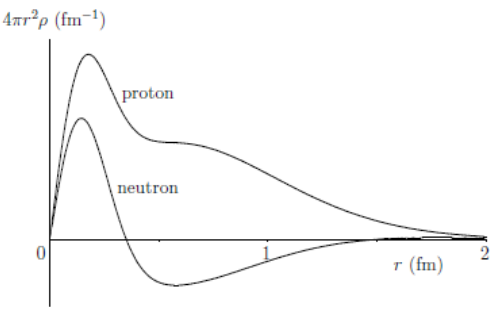
\includegraphics[scale=0.35]{ch1/image2.png}
	\captionof{figure}{ }
	\end{wrapfigure}
Le nucléon est un fermion, son spin vaut donc $1/2$. De plus, comme sa densité de charge n'est pas 
constante, il ne s'agit pas d'une particule élémentaire. Cependant, nous avons que
\begin{equation}
\left\{\begin{array}{ll}
\DS \int \rho_p(r)dr &=1\\
\DS \int \rho_n(r)dr &=0
\end{array}\right.
\end{equation}
Il est alors possible de déterminer le rayon de charge du proton
\begin{equation}
<r^2>_p = \int \rho_p(r)^2\ dr \quad\Leftrightarrow\quad <r^2>_p^{1/2} = 0.87\ \text{fm}
\end{equation}
Le fait que le neutron ne soit pas une particule élémentaire a poussé à introduire le quark 
(de spin $1/2$) : le quark \textit{up} d'une charge de $2/3e$ et le \textit{down} d'une charge
de $-e/3$. Un proton est alors le mélange de quarks \textit{uud} alors que le neutron est \textit{udd}.



\section{Types de particules (et antiparticules)}
Il existe deux grand types de particules : les \textit{leptons} et les \textit{hadrons}.
\begin{enumerate}
\item Les leptons sont des particules élémentaires de charges $-e$ et de spin $1/2$
	\begin{itemize}
	\item[$\bullet$] $e^-, \mu, \tau + \nu$
	\end{itemize}
\item Les hadrons sont composés de quarks ($u,d,s,c,b,t$)
	\begin{itemize}
	\item[$\bullet$] Les \textit{baryons} sont formés de 3 quarks (comme le nucléon)
	\item[$\bullet$] Les \textit{mésons} sont formés d'un quark et d'un antiquark (comme le pion)
	\end{itemize}
\end{enumerate}

	\subsection{Les baryons (spin $1/2$)}
	Ceux-ci sont formés de trois quarks parmi $u,d$ et $s$. Le couplage de deux spins $1/2$ impose
	que $S_{12}$ soit 0 ou 1 (deux possibilités). L'ajout d'un troisième spin $1/2$ augmente le 
	nombre de possibilités à six, il y a donc huit particules possibles. \\
	 
	 Le principe d'exclusion de Pauli interdit les combinaisons de quarks $uuu, ddd$ ou $sss$ car 
	 si trois particules sont du mêmes types, elles doivent avoir des états différents ce qui n'est 
	 pas le cas ici. 
	  
 	 \notes{Considérons le vecteur cinétique $\vec{j_1} = (j_{1x}, j_{1y},j_{1z})$ avec $j_1^2= j_{1x}^2+
 	 j_{1y}^2+j_{1z}^2$. L'opérateur moment cinétique est alors défini par son application sur 
 	 le \textit{ket} $\ket{jm}$ : $J_1^2\ket{jm} = j(j+1)\ket{jm}$. \\
 	 
 	 Il est possible de coupler le moment cinétique $\vec{J} = \vec{j_1}+\vec{j_2}$
 	 \begin{equation}
 	 \vec{J}^2\ket{JM} = J(J+1-\ket{JM}\qquad \text{où }\ |j_1-j_2|\leq J\leq j_1+j_2
 	 \end{equation}
 	 Par exemple, pour l'électron de moment cinétique $l$ et de spin $1/2$, nous avons que 
 	 $|l-1/2| \leq j \leq l+1/2$. Tentons de comprendre les possbilités de baryons en considérant le 
 	 couplage de deux nucléons
 	 \begin{equation}
 	 \left.\begin{array}{ll}
 	 s_n &= 1/2\\
 	 s_p &= 1/2 
 	 \end{array}\right\}\to S_{12} = 0,1\quad\text{ car }\quad 0\leq S_{12} \leq 1\quad\text{ et }\quad
 	 S_{12}\in\mathbb{Z}
 	 \end{equation}
 	 Effectuons maintenant le couplage du troisième spin $1/2$. Comme $-j\leq m \leq j$, nous avons
 	 $2j+1$ possibilités. Ainsi pour $S_{12}=0,1$, $M_S=0$ pour $S_{12}=0$ et $M_S=-1,0,1$ pour 
 	 $S_{12}=1$. L'ajout du troisième spin offre donc six nouvelles possibilités.}

	\subsection{Les mésons (spin $0$)}
	Ceux-ci sont formés d'un quark et d'un antiquark parmi $u,d$ et $s$ ce qui offre neuf particules
	possibles (dont le kaon $K$ et le pion $\pi$). Ils ont une durée de vie de l'ordre de $10^{-8}$ s.
\newpage


\section{Types de forces}
Il existe quatre types de forces
\begin{enumerate}
\item Nucléaire forte, attractive et de courte portée
\item Nucléaire faible, de portée\dots faible
\item Électromagnétique, de portée infinie
\item Gravitationnelle, de portée infinie. Bien que son amplitude soit très faible, les masses énormes
(comme la masse terrestre) compense ceci.
\end{enumerate}
L'hamiltonien d'un noyau s'écrit
\begin{equation}
H = \sum_i T_i + \sum_{ij} V_{ij}
\end{equation}
où le premier terme est l'énergie cinétique et le second terme l'interaction nucléon-nucléon composée 
de deux termes : $V_{ij} = V_N+V_C$ où $V_N$ est d'origine nucléaire (pas connue exactement même si on 
le sait attractif et de courte portée) et $V_C$ l'origine coulombienne (nulle pour un neutron-neutron ou 
neutron-proton et valant $e^2/r$ pour un proton-proton).\\

Le problème est que ceci est difficilement résolvable même numériquement (l'interaction nucléaire n'étant
pas parfaitement connue), il faudra donc recourir à l'utilisation de modèles.

